\documentclass[amsmath,amssymb,11pt]{article}
\usepackage[utf8]{inputenc}
\usepackage{amsmath}
\usepackage{amsmath,amsopn}
\usepackage{xcolor}
\usepackage{tikz}
\usetikzlibrary{snakes}

\begin{document}

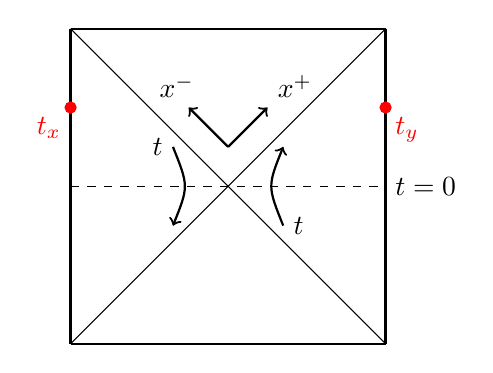
\begin{tikzpicture}


\draw[thick] (0,0) -- (4,0);
\draw[thick] (0,0) -- (0,4);
\draw[thick] (0,4) -- (4,4);
\draw[thick] (4,0) -- (4,4);
\draw (0,0) -- (4,4);
\draw (0,4) -- (4,0);

\draw[->,thick] (2,2.5) -- (2.5,3) node[above right]{$x^+$};
\draw[->,thick] (2,2.5) -- (1.5,3) node[xshift=.2cm,above left]{$x^-$};


\filldraw[red] (0,3) circle (2pt) node[anchor=north east]{$t_x$};
\filldraw[red] (4,3) circle (2pt) node[anchor=north west]{$t_y$};

\draw[dashed] (0,2) -- (4,2) node[pos=1,right]{$t=0$};

\draw[->,thick] (2.7,1.5) .. controls (2.5,2) .. (2.7,2.5) node[pos=0,right]{$t$};
\draw[<-,thick] (1.3,1.5) .. controls (1.5,2) .. (1.3,2.5) node[pos=1,left]{$t$};

\end{tikzpicture}

\end{document}